\documentclass[12pt]{mcmthesis}
\mcmsetup{CTeX = false,
    tcn = {12833},  %% your team control number
    problem = {B}, %% your chosen problem (A or B)
    sheet = true,
    titleinsheet = True,
    keywordsinsheet = true,
    titlepage = false,
    abstract = false}

\usepackage{newtxtext}%\usepackage{palatino}
\usepackage{comment}
\usepackage{lipsum}
\hypersetup{
    colorlinks=false,
    linkcolor=blue,
    filecolor=blue,
    urlcolor=blue,
    citecolor=cyan,
}
\usepackage{color}
\usepackage{float}
\numberwithin{figure}{section}
\numberwithin{table}{section}
\numberwithin{equation}{section}
\usepackage{enumerate}

\usepackage{placeins}
\usepackage[figuresright]{rotating}
\usepackage[final]{pdfpages}
%\usepackage[
%    backend=bibtex,
%    style=numeric-verb,
%]{biblatex}
\usepackage{babel}
\usepackage{textcomp}
\usepackage{changepage}
\usepackage{siunitx}
\usepackage{lstmisc}
\usepackage{booktabs}
\usepackage{blindtext}
\usepackage{capt-of}
\usepackage{algorithm}
\usepackage{algorithmicx}
\usepackage{algpseudocodex}
\usepackage{tocloft}
\usepackage{sansmathfonts}
\usepackage[T1]{fontenc}
\renewcommand*\familydefault{\sfdefault}

\renewcommand*\familydefault{\sfdefault}


%\addbibresource{citations.bib}


%! suppress = LineBreak
\begin{document}
    \graphicspath{ {./figs/} }

    \setlength{\abovedisplayskip}{3pt}
    \setlength{\belowdisplayskip}{3pt}
    \setlength{\abovedisplayshortskip}{-12pt}
    \setlength{\belowdisplayshortskip}{0pt}

    \setlength{\abovecaptionskip}{0pt}

    \title{Quantitatively Modelling CO\textsubscript{2} and Global Warming}


    \begin{abstract}
        Abstract

        \begin{keywords}
            Global Warming, Greenhouse Gases, CO\textsubscript{2}, Forecast, Predictions, Environment, Temperature
        \end{keywords}

    \end{abstract}

    \maketitle

    \setcounter{page}{2}

    \setlength{\cftparskip}{0pt}
%    \renewcommand{\baselinestretch}{0}\normalsize
    \tableofcontents
%    \renewcommand{\baselinestretch}{0.8}\normalsize

    \newpage


    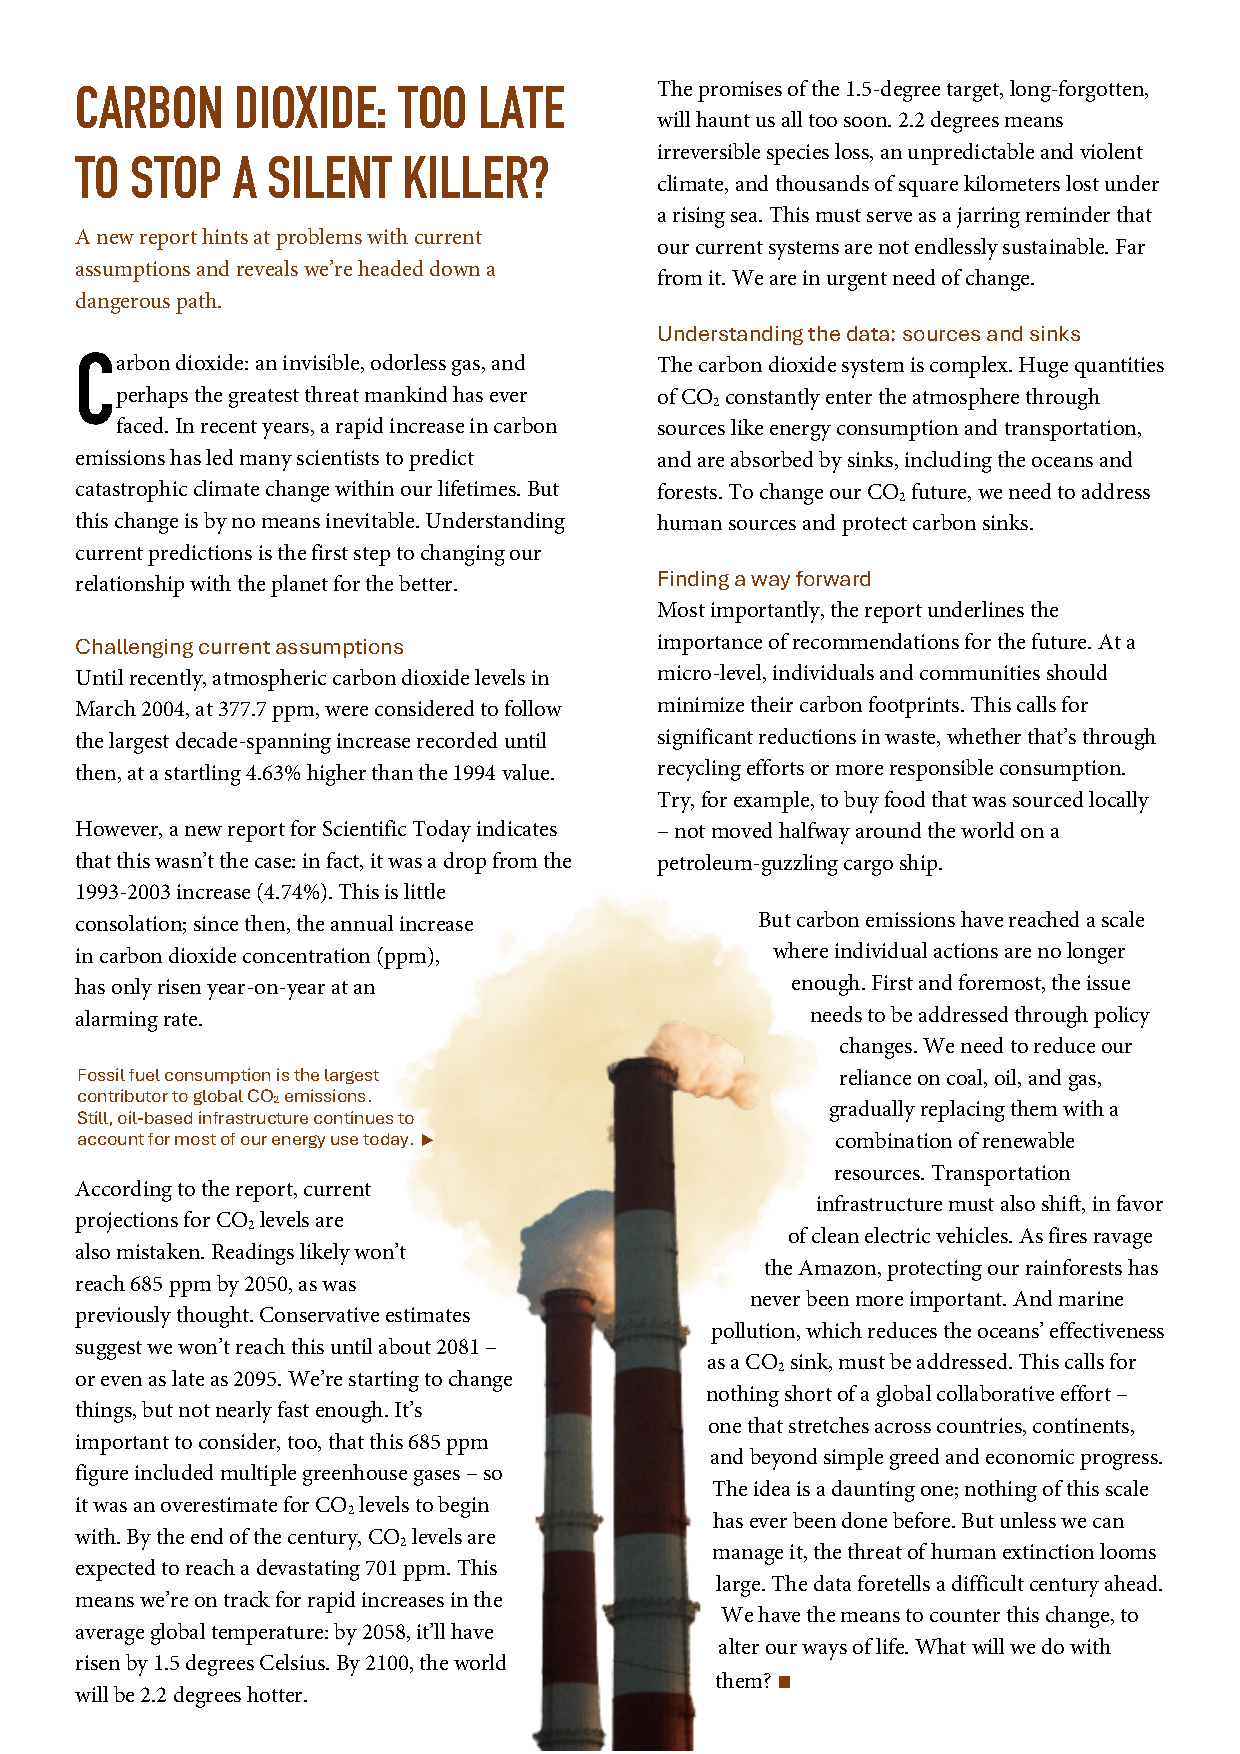
\includepdf[
        pages=-,
        addtotoc={1,section,1,New Report,a1}
    ]{article.pdf}


    \section{Introduction}

    \subsection{Background}
    The most significant greenhouse gas on Earth is carbon dioxide, which both absorbs and radiates heat. In contrast to oxygen and nitrogen, which together make up the majority of our atmosphere, greenhouse gases absorb heat emitted from the Earth's surface and re-emit it in all directions, including back toward the planet's surface. The natural greenhouse effect that keeps the Earth's atmosphere above freezing would be insufficient without carbon dioxide. People are accelerating the natural greenhouse effect and raising the earth's temperature by releasing more carbon dioxide into the atmosphere. The NOAA Global Monitoring Lab found that in 2021, carbon dioxide accounted for nearly two thirds of the total heating influence of all greenhouse gases created by humans.

    Prior to the Industrial Revolution, carbon dioxide in the atmosphere was consistently around 280 parts per million (ppm).
    The concentration of CO\textsubscript{2} in the atmosphere reached 377.7 ppm in March 2004, resulting in the largest 10-year average increase up to that time.
    According to scientists from National Oceanographic and Atmospheric Administration (NOAA) and Scripps Institution of Oceanography (SIO) the monthly mean CO\textsubscript{2} concentration level peaked at 421 ppm in May 2022.
    An Organisation for Economic Co-Operations and Development (OECD) report predicts a CO\textsubscript{2} level of 685 ppm by 2050.

    \subsection{Problem Analysis}
    \noindent\textbf{Problem 1: CO\textsubscript{2} level Forecasting}

    \begin{adjustwidth}{1cm}{}

        \noindent Modelling.

        \vspace{-6pt}
        \noindent Prodice models that reflect existing CO\textsubscript{2} data and extrapolates to reasonable predictions.

        \begin{adjustwidth}{1cm}{}
            \noindent Choose suitable mathematical models and fit each one to existing data.

            \noindent Evaluate each model\ldots~
            Use different evaluation approaches including statistical accuracy, contextual reasoning, comparison with external predictions, etc.

            \noindent Generate a conclusive model based on results obtained\ldots~
            Either pick the ``best'' model, or create new model based on multiple sub-parts.
        \end{adjustwidth}

        \noindent Verify External Claims.

        \begin{adjustwidth}{1cm}{}
            \noindent Whether CO\textsubscript{2} levels in 2004 had a ``larger increase than observed over any previous 10-year period''.

            \begin{adjustwidth}{1cm}{}
                \noindent Determine how exactly the comparison is done with ``any previous 10-year period''\ldots~
                Find supporting evidence from existing literature or make the best interpretation.
            \end{adjustwidth}

            \noindent Whether CO\textsubscript{2} levels will reach 685ppm by 2050.

            \begin{adjustwidth}{1cm}{}
                \noindent Testify this statement against all models.
            \end{adjustwidth}

        \end{adjustwidth}

        \noindent Draw Conclusions.

        \vspace{-6pt}
        \noindent Real-world implications based on predictions and results.

    \end{adjustwidth}


    \noindent\textbf{Problem 2: Temperature vs CO\textsubscript{2}}

    \begin{adjustwidth}{1cm}{}

        \noindent Modelling.

        \vspace{-6pt}
        \noindent Produce models that reflect existing temperature data and extrapolates to reasonable predictions.

        \begin{adjustwidth}{1cm}{}
            \noindent Direct relationship between CO\textsubscript{2} and temperature.

            \noindent Temperature as a time series, and compare with CO\textsubscript{2} models from Problem 1.
        \end{adjustwidth}

        \noindent Predictions.

        \vspace{-6pt}
        \noindent Predict points in time where global temperature will have an average increase of 1.25\textdegree C, 1.5\textdegree C, and 2\textdegree C compared to the base period of 1951--1980.

        \noindent Evaluation.

        \vspace{-6pt}
        \noindent Longevity \& Confidence; discuss the distance into the future that the model can still predict with reasonable accuracy.


    \end{adjustwidth}

    \bigskip

    \noindent Our thought process and plan is presented here below as a flowchart:
    \begin{center}
        \makebox[\textwidth]{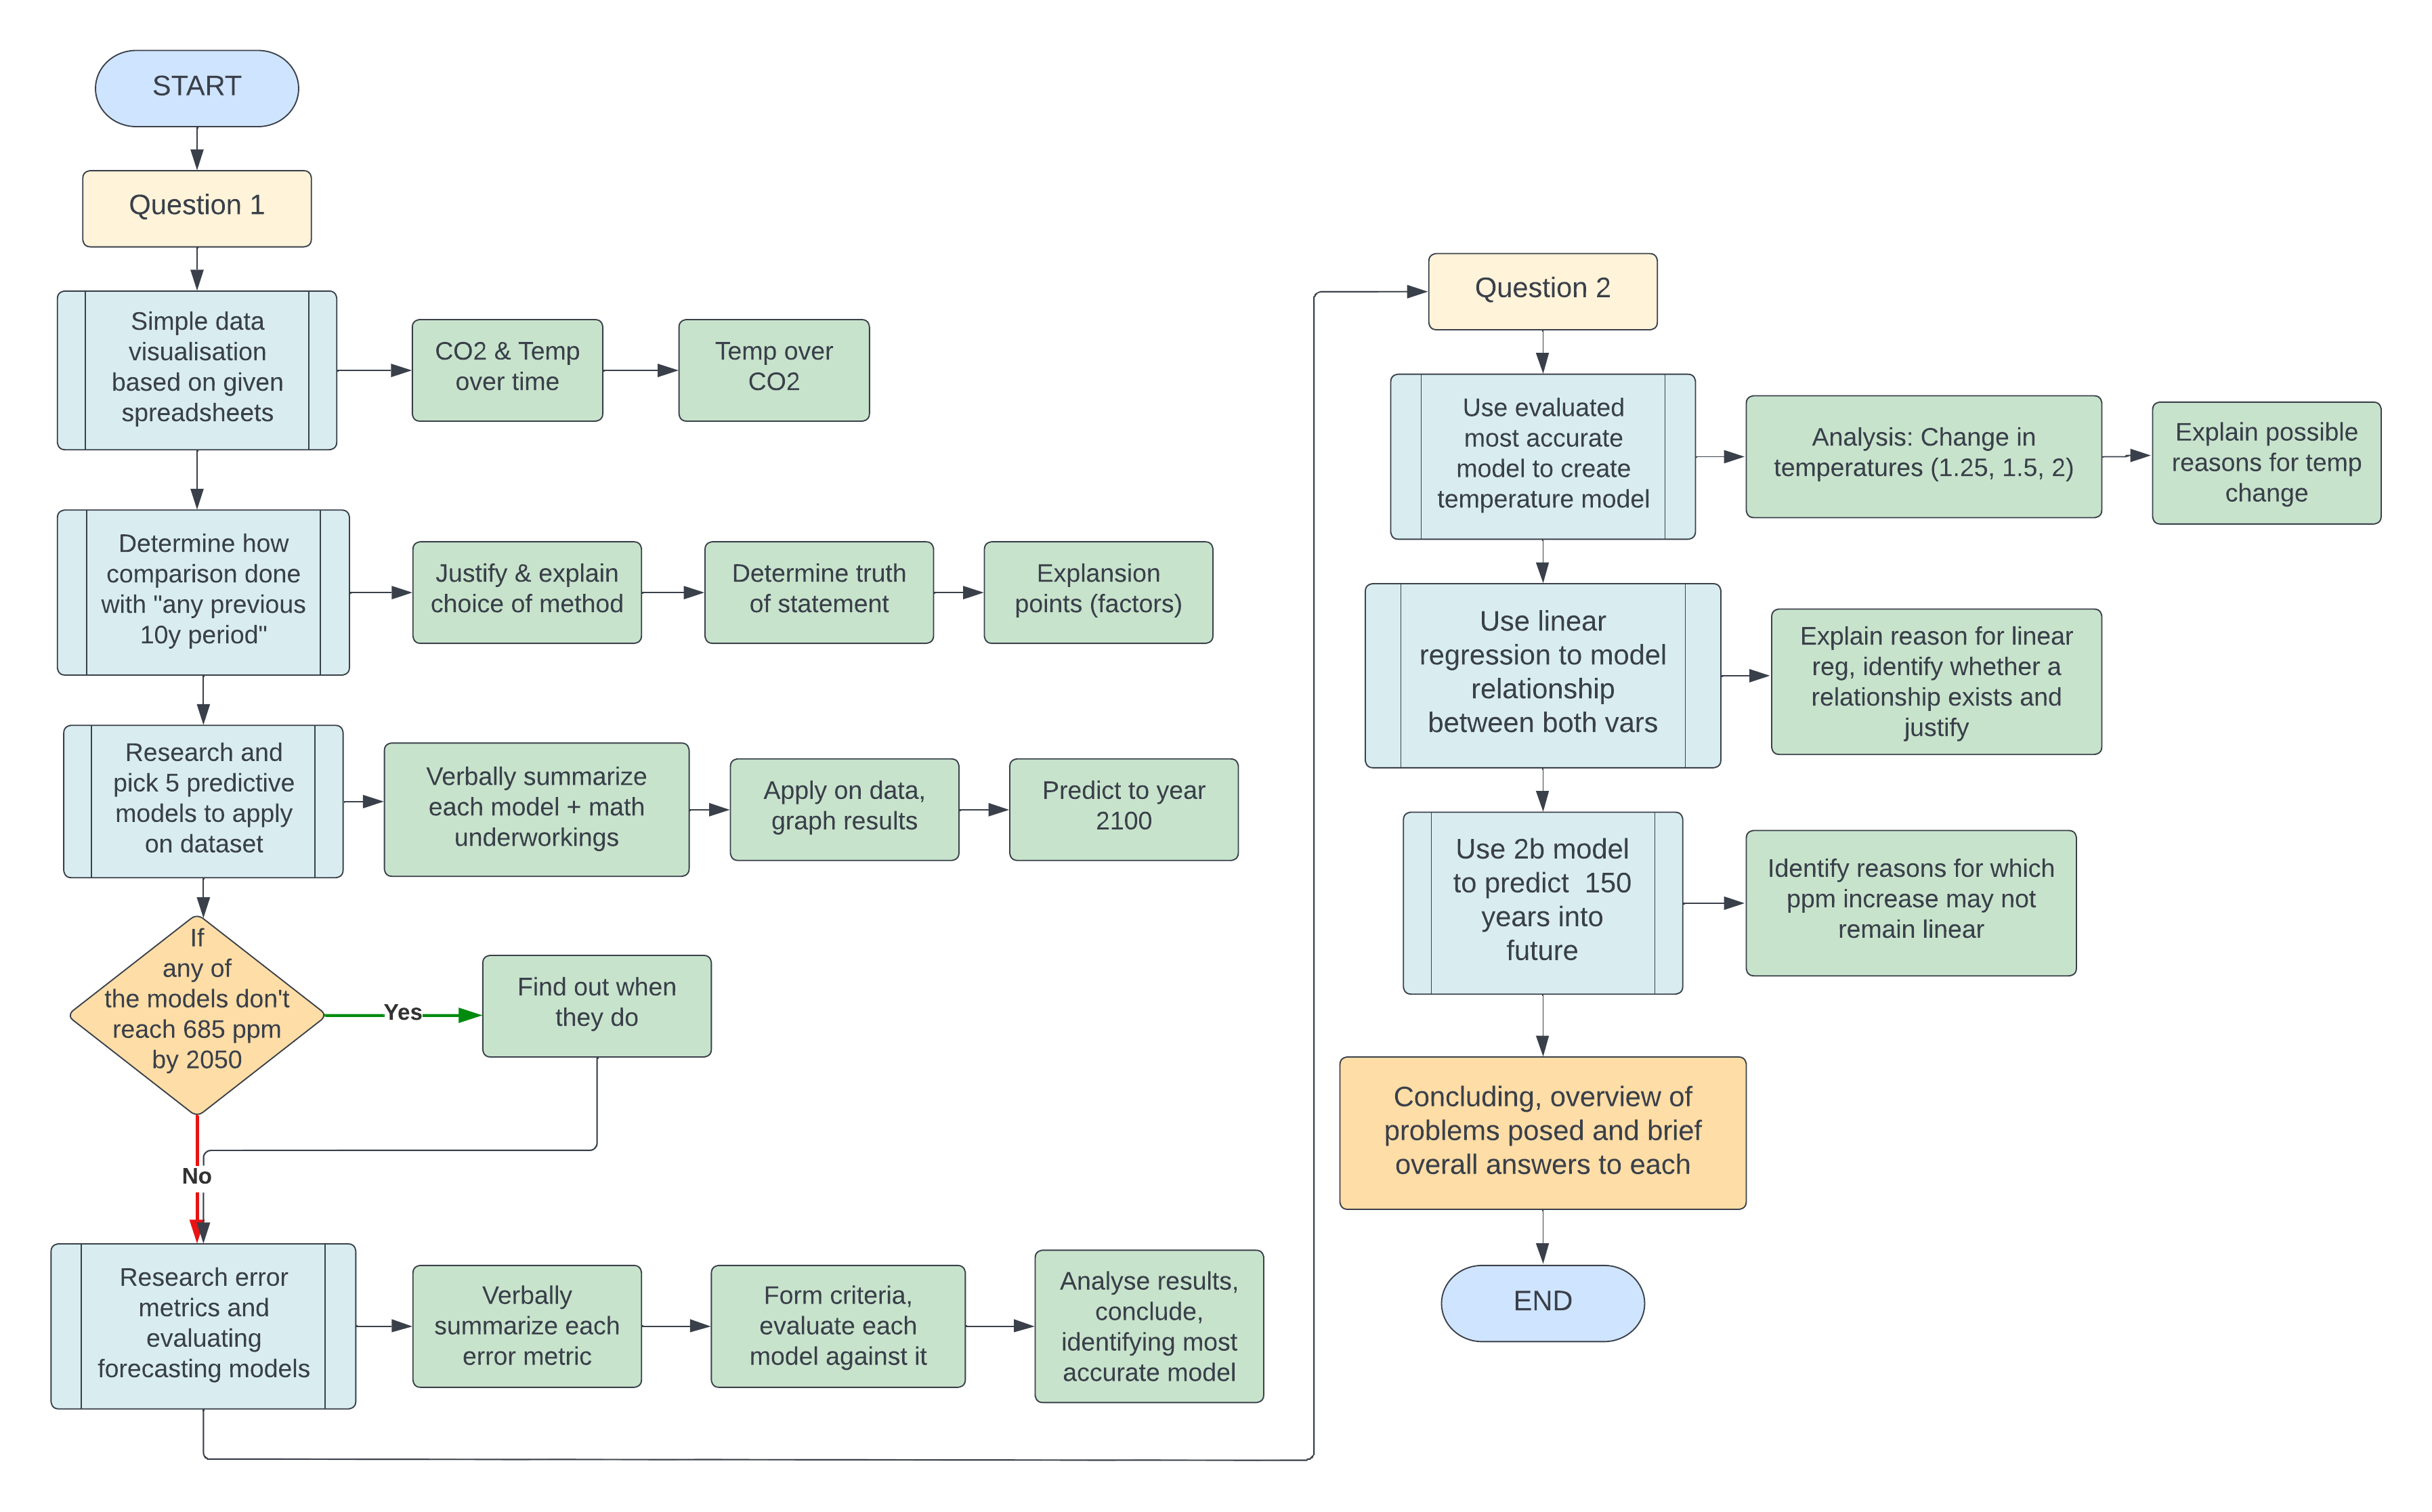
\includegraphics[width=\textwidth]{plan}}
    \end{center}

    \subsection{Keyword Definitions}
    \noindent\textbf{CO\textsubscript{2} Level/Content}: Global average concentration of CO\textsubscript{2} in the atmosphere, in parts-per-million (ppm).

    \noindent\textbf{Relative Temperature}: Global average temperature, relative to the baseline average temperature from 1951 to 1980, in degrees Celsius.

    \noindent\textbf{Error Metric Abbreviations}: See Table~\ref{tab:err_abb}.

    \begin{table}[H]
        \centering
        \begin{tabular}{ll}
            \toprule
            Abb.                 & Full                                         \\
            \midrule
            MSE                  & Mean Squared-Error                           \\
            RMSE                 & Square root of MSE                           \\
            MAE                  & Mean Absolute Error                          \\
            PCC                  & Pearson's Correlation Coefficient            \\
            R\textsuperscript{2} & Coefficient of Determination, or PCC Squared \\
            CVAR                 & Covariance                                   \\
            \bottomrule
        \end{tabular}
        \vspace{8pt}
        \caption{Abbreviations of Error Metrics}
        \label{tab:err_abb}
    \end{table}

    \subsection{Assumptions and Justifications}
    \noindent\textbf{Assumption 1}: CO\textsubscript{2}, as a greenhouse gas, has a true case-and-effect relationship with temperature.

    \vspace{-6pt}
    \noindent\textbf{Justification}: Most existing literature and evidence suggest that CO\textsubscript{2} is a greenhouse gas, and that greenhouse gases traps heat and leads to increases in temperature on a global scale. This fact is taken for granted to make more confident predictions that relate temperature to CO\textsubscript{2} levels.

    \noindent\textbf{Assumption 2}: Both datasets provided for CO\textsubscript{2} emissions and temperatures are reliable and accurate.

    \vspace{-6pt}
    \noindent\textbf{Justification}: Accurate predictions are always based on accurate data. Since official data is given along the problem, they will be taken and treated assuming the absence of mistakes and errors.

    \subsection{General Variables}
    See table~\ref{tab:my_label}:

    \begin{table}[h!]
        \centering
        \begin{tabular}{cc}
            \toprule
            Variable   & Definition                                                 \\
            \midrule
            $C_i$      & CO\textsubscript{2} level at year $i$                      \\
            $T_i$      & Temperature at year $i$                                    \\
            $C^{-1}_i$ & Year where (predicted) CO\textsubscript{2} is at level $i$ \\
            $T^{-1}_i$ & Year where (predicted) Temperature is at $i$               \\
            \bottomrule
        \end{tabular}
        \vspace{8pt}
        \caption{General Variables}
        \label{tab:my_label}
    \end{table}


    \section{The Generic Modelling Procedure}
    In this section, the generic procedure to produce specific models for a given task is stated and explained. All relevant information; such as metrics, concepts, and terms; are explained and directly referred to later. This section helps avoid bloat in the paper by isolating generic baseline information to prevent repetition and confusion.

    \subsection*{Modelling, Conceptually}

    ``A mathematical model is a description of a \textit{system} using mathematical concepts and language.'' (wikipedia reference) A completed math model should describe/simulate it\textquotesingle s target system to the best of its ability. All models behave like a (complex) function~\eqref{eq:model_func} - it produces outputs when given inputs. For this problem, the \textit{system}s to be modelled are atmospheric CO\textsubscript{2} and global warming.
%
    \begin{equation}
        y = f(x)
        \label{eq:model_func}
    \end{equation}
%
    \noindent where $y$ is the output, $x$ is the input, and $f$ is the model itself.

    \subsection*{Time Series}

    Inputs and outputs differ depending on the type of the model, but one type relevant to this paper is are time-series\textquotesingle . In a time-series model, the input is a timeframe, and the output describes the state of a system it is modelling; conceptually, a time-series models the evolution of a possibly boundless dynamic system over time~\eqref{eq:model_ts}. This will be useful later to, for example, model the change of CO\textsubscript{2} levels over time. Time-series\textquotesingle~belong to the family of relationship models, which produces outputs based on an input variable, effectively translation values between two variables. This will be useful later to model the relationship between CO\textsubscript{2} levels and temperature change.
%
    \begin{equation}
        \begin{aligned}
            t & \rightarrow y \\
            \Delta t & \rightarrow \Delta y + y_0
        \end{aligned}
        \label{eq:model_ts}
    \end{equation}
%
    \noindent where $y$ is the output, $t$ is the time or input, and $y_0$ is the initial state (when modelling relative evolution over time).

    \subsection*{Quantitative Data}

    Because math models are strictly quantitative, a pre-defined procedure must exist to translate between real-world parameters and numeric values. For most systems, this can be done using existing scientific measurements and units. Otherwise, custom metrics have to be defined. With the given problem, there are simple metrics for both CO\textsubscript{2} levels in the atmosphere and global warming, concentration in parts-per-million and temperature in degrees Celsius, respectively. In terms of time, years are already represented numerically.

    Once the system can be represented quantitatively and a quantitative output can be interpreted as a state of the system, a math model can be constructed. There are many different approaches to construct a model from numerical representations of a system, but this paper focuses on ``fitting'' ``generic models'' to true/historical numeric data.

    \subsection*{Function Regression}

    In short, a ``generic model'' is a mathematical function parameterized by a variable amount of constants within its definition~\eqref{eq:model_g}. The function exhibits specific characteristics regardless of the values of its parameters. The end goal of modelling is to adjust these parameters such that the function can produce the most accurate output (compared to the real system) for each given input. In the case of modelling CO\textsubscript{2} levels as a time-series, the model function should produce ppm values for a given year.
%
    \begin{equation}
        \begin{aligned}
            \bm{\beta} &= [p_1, p_2, p_3, p_4, \dots] \\
            f(x) &= g(x, \bm{\beta}) \\
            y &= f(x)
        \end{aligned}
        \label{eq:model_g}
    \end{equation}
%
    \noindent where $g$ is the generic model, and $f$ is a constructed model by finding specific values for each of the parameters $p_i$. $\bm{\beta}$ is simply a vector that encapsulates all of the parameters.

    \subsection*{Error Metrics}

    ``Fitting'' a model, also known as ``optimization'', is a systematic approach to find parameters that ``best'' models the given system. Usually, an error function is defined to quantitatively gauge how accurate or good the model is by calculating a metric based on the difference between the actual output and expected output for a given input~\eqref{eq:model_diff}. The optimization process tries to produce the ``best'' model by minimizing the error function across all available data values. For example,~\eqref{eq:model_sqd} is a square-error function that gives the sum of square-errors for all data points.
%
    \begin{equation}
        E(y) \approx y - \hat y
        \label{eq:model_diff}
    \end{equation}

    \begin{equation}
        E_{sum} = \sum_{i=1}^{n} (f(x_i) - \hat y_i)^2
        \label{eq:model_sqd}
    \end{equation}

    \subsection*{Optimization}

    The optimization process aims to minimize the (sum of the) error function.
    A generic approach is to take partial derivatives of the summed error with respect to every parameter in the model. This allows the minimum to be calculated by equating the differential functions to 0.
    Generally, the partial derivative of error $E$ with respect to parameter $\beta_j$ is:
%
    \begin{equation}
        \begin{aligned}
            \frac{\partial E}{\partial \beta_j} &= 2 \sum_i e_i \frac{\partial e_i}{\partial \beta_j} \\
            \frac{\partial E}{\partial \beta_j} &= -2\sum_i e_i\frac{\partial f(x_i,\boldsymbol \beta)}{\partial \beta_j}
        \end{aligned}
    \end{equation}
%
    \noindent where $e$ is the error, and $j = 1, \ldots, m$ for $m$ parameters in $\beta$.



    \section{CO\textsubscript{2} - Modelling}
    This section includes a walk through of all mathematical models used to model the CO\textsubscript{2} levels as a time series and how they specifically apply to the given data.

    \subsection{Pre-Analysis}
    Firstly, this problem takes the form of a single-variable time series; CO\textsubscript{2} levels evolve as time passes, and we are trying to model the relationship between time and CO\textsubscript{2}.
    Based on simple logic and scientific reasoning, there is no cause-and-effect relationship between time and carbon dioxide levels, so the models will assume a relationship that is purely a statistical correlation.

    The given CO\textsubscript{2} data is graphed to visualize the rough correlation and trend present in the data -~\ref{fig:co2}. It is very apparent that there is a strong correlation with minimal variance between time and carbon dioxide levels. The shape of the curve seems exponential. These ideas will be help guide future mathematical modelling.
    Auto-correlation is calculated to identify any seasonality within the data -~\ref{fig:co2_acf}. However, it is apparent that there is no clear seasonality within the data, as shown by the lack of an oscillating correlation. This is expected since the data comes in annual resolutions; yearly seasonality could be expected due to seasonal effects, but would only be observed with monthly data.

    \begin{figure}[h]
        \centering
        \begin{minipage}{.5\textwidth}
            \centering
            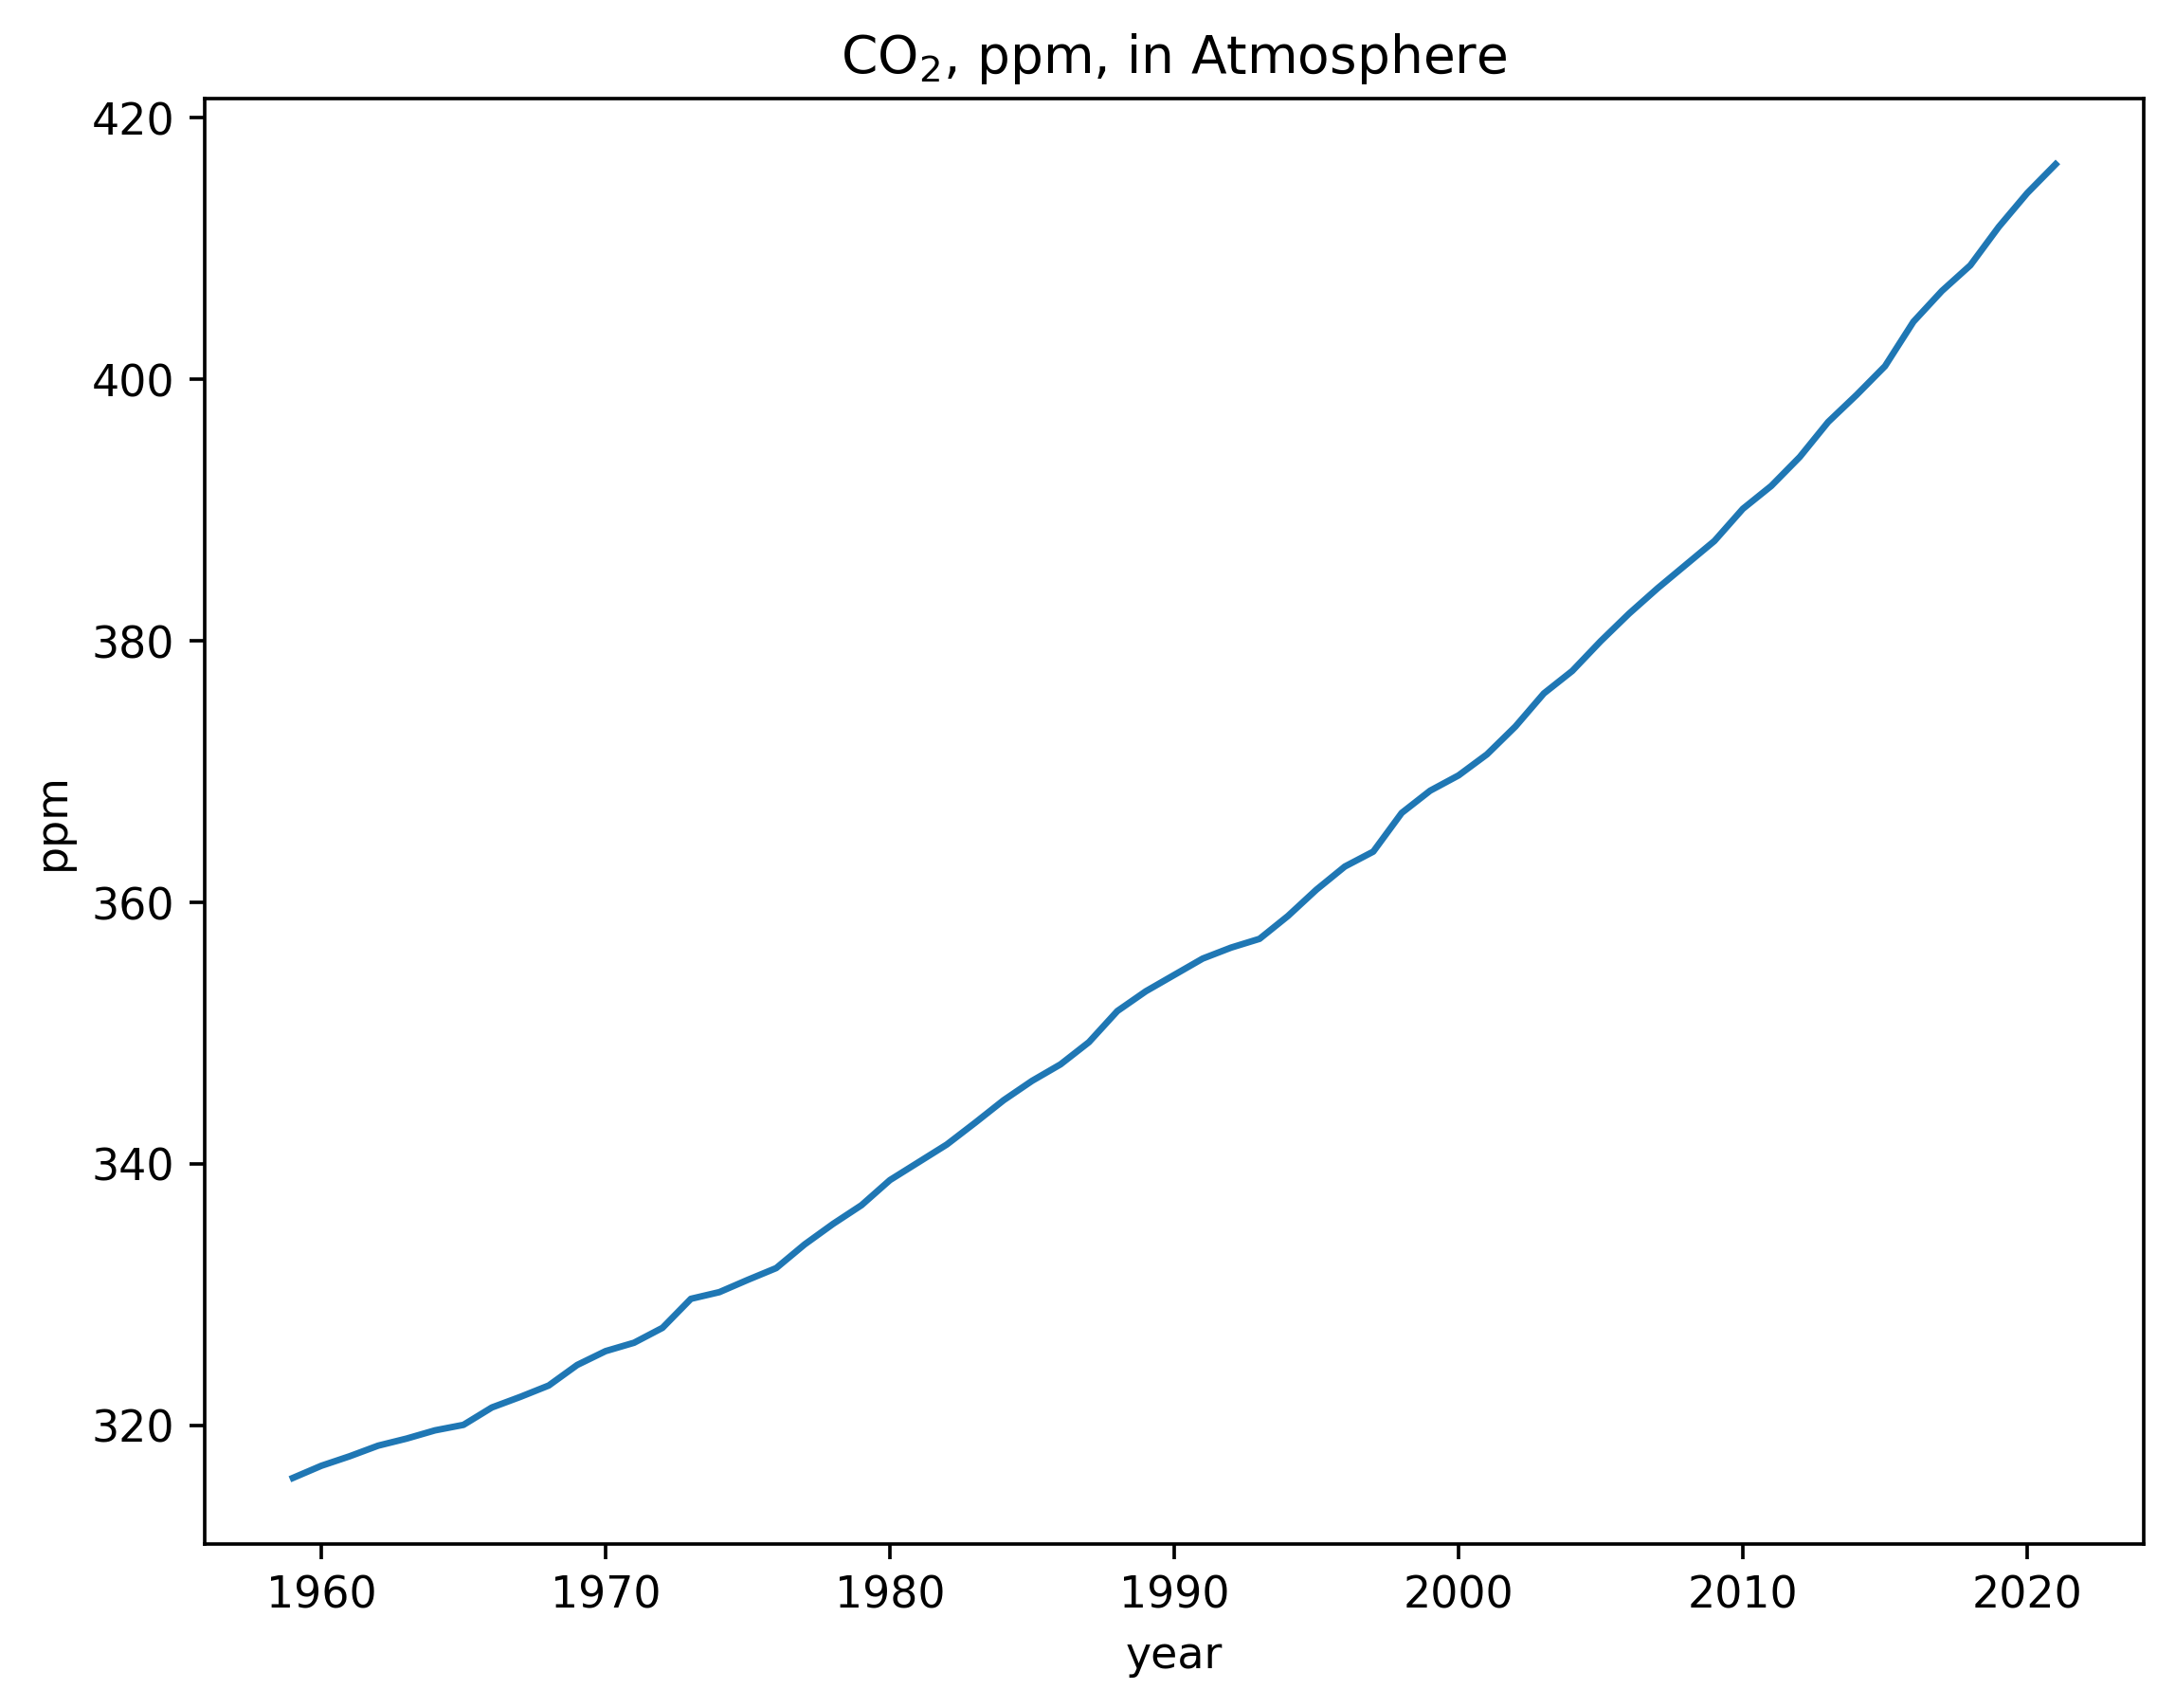
\includegraphics[width=\textwidth]{co2}%
            \caption{Graph of given CO\textsubscript{2} data}
            \label{fig:co2}
        \end{minipage}%
        \begin{minipage}{.5\textwidth}
            \centering
            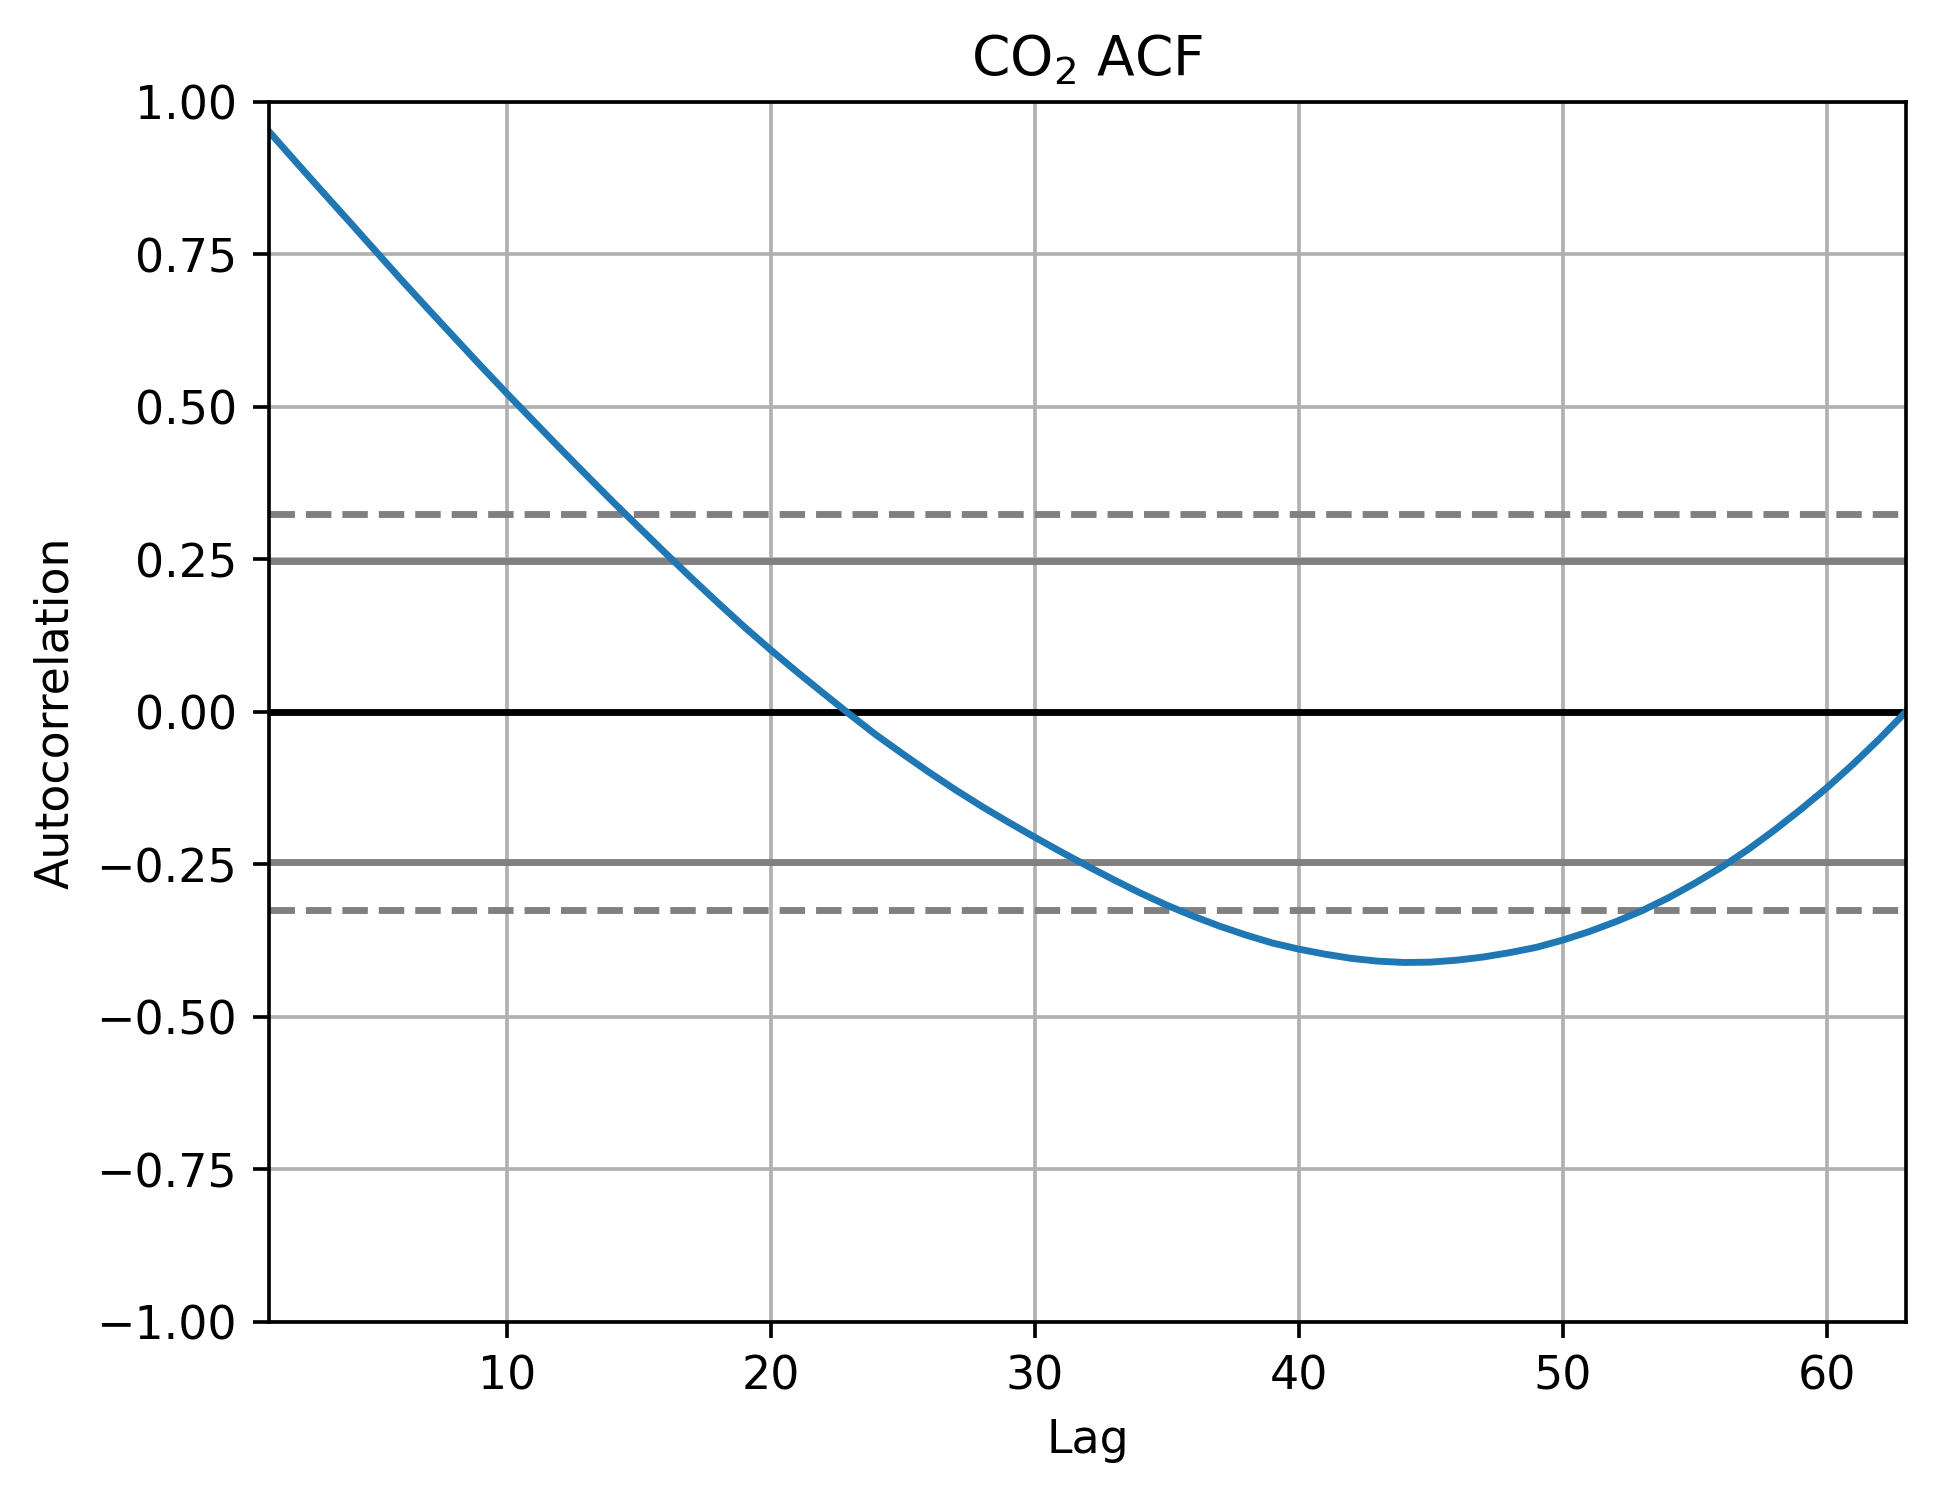
\includegraphics[width=\textwidth]{co2_acf}%
            \caption{CO\textsubscript{2} Auto-correlation}
            \label{fig:co2_acf}
        \end{minipage}
    \end{figure}

    \subsection{Linear}
    A linear regression is performed first due to its simplicity and ability to help pick more complex models.

    Linear regression is an approach used to model a linear relationship between an independent variable $x$ and a dependent variable $y$ by finding the slope of the trend and initial value ($y$ when $x$ is 0).
    It is used to represent existing data and predict future values; linear models are used both for interpolation and extrapolation. In this case, the model will be fit to existing data and used to predict future CO\textsubscript{2} levels.
    A linear growth function takes the general form of~\eqref{eq:lr}:
%
    \begin{equation}
        f(x) = \alpha x = \beta
        \label{eq:lr}
    \end{equation}
%
    \noindent where $\alpha$ is the coefficient, or growth rate; and $\beta$ is the y-intercept, or initial value.
    The values of $\alpha$ and $\beta$ are ``optimized'' using an algorithm to model a given dataset with the minimum ``error''.

    One of the most common and simplest methods used to calculate the coefficient and intercept of the regression line is the Ordinary Least Square (OLS) \textit{optimization} method.
    In short, OLS minimizes the Square-Error for each point against a given linear function by adjusting the function\textquotesingle s parameters, which in the end produces optimal parameters for a equation in the form of a linear line of best fit.

    The Square-\textit{Error} function, which is what OLS \textit{optimizes}, is simply a summation of the squares of the difference between actual values and predicted values, over all data points~\eqref{eq:ls}:

    \begin{equation}
        E = \sum{(y - \hat{y})^2}
        \label{eq:ls}
    \end{equation}

    Because the predicted values $\hat{y}$ for a linear model is modelled as $\alpha x + \beta$, the Square-Error function for a linear model can be more specific~\eqref{eq:ls_lr}:

    \begin{equation}
        E = \sum{(y - (\alpha x - \beta))^2}
        \label{eq:ls_lr}
    \end{equation}

    OLS calculates the values of $\alpha$ and $\beta$ which minimize $S$ in the summation above.
    Unlike the generic differential method described above, OLS is specialized for linear functions and can calculate the optimal parameters in one stop, using summation ratios.
    The coefficient $\alpha$, or the linear trend of the dataset can be calculated with~\eqref{eq:lr_coef}:

    \begin{equation}
        \alpha = \frac{n \sum x_i y_i - \sum x_i \sum y_i }{n \sum x^2_i - (\sum x_i)^2}
        \label{eq:lr_coef}
    \end{equation}

    \noindent where $n$ is the number of data points.

    After calculating the slope of the trend, the intercept $\beta$, is calculated by~\eqref{eq:lr_intc}:
%
    \begin{equation}
        \beta = \bar y - \alpha \bar x
        \label{eq:lr_intc}
    \end{equation}

    OSL was applied to the given data set to obtain the coefficient $\alpha$ and the y-intercept $\beta$ - $1.6140361$ and $2854.59326421$, respectively - which corresponds to the following linear equation:
%
    \begin{equation}
        C_i = 1.6140361 i - 2854.59326421
        \label{eq:co2_lr}
    \end{equation}
%
    \noindent where $i$ is the year.

    The inverse of the function is derived by solving for $i$ in terms of $C$:

    \begin{equation}
        C^{-1}_i = \frac{C + 2854.59326421}{1.6140361}
        \label{eq:co2_lr_inv}
    \end{equation}

    $C$ was then set to 685 to find the year at which CO\textsubscript{2} emissions would reach 685ppm; it was found that it would reach this level at the year 2193.
    The regression line was then graphed and used to predict the next 30 years of CO\textsubscript{2} emissions; the actual data is also plotted for comparison (Fig.~\ref{fig:co2_lr}).


    Linear regression is useful in relation to the problem as it is simple to interpret and portray, allowing the prediction of data to be accurate during interpolation.
    However, if the data to be predicted is outside of the range, such as predicting future CO\textsubscript{2} levels, extrapolation may be inaccurate due to a false assumption of the trend.
    Furthermore, if the variables plotted provide a non-linear relationship, a linear regression line may inaccurately represent and predict values, which is the case in the data provided.
    Statistical error of the linear regression model against existing data shows a good but not perfect accuracy (Table~\ref{tab:co2_lr_err}).

    \begin{table}[h]
        \begin{minipage}{0.7\linewidth}
            \centering
            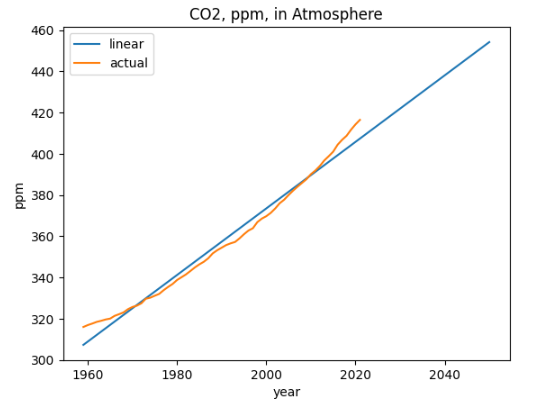
\includegraphics[width=\textwidth]{linear}%
            \captionof{figure}{Graph of given CO\textsubscript{2} data}
            \label{fig:co2_lr}
        \end{minipage}%
        \begin{minipage}{0.3\linewidth}
            \centering
            \begin{tabular}{ll}
                \toprule
                Metric               & Value  \\
                \midrule
                MSE                  & 15.376 \\
                RMSE                 & 3.9212 \\
                MAE                  & 3.1920 \\
                PCC                  & 0.9912 \\
                R\textsuperscript{2} & 0.9825 \\
                CVAR                 & 875.32 \\
                \bottomrule
            \end{tabular}
            \vspace{8pt}
            \caption{Error Metrics for Linear Regression}
            \label{tab:co2_lr_err}
        \end{minipage}
    \end{table}

    \subsection{Exponential}
    The second approach decided upon was exponential regression, which models the non-linear relationship between an independent variable $x$ and dependent variable $y$, where the rate of change of $y$ with respect to $x$ at a given point is proportional to the quantity itself.
    This choice was made based on visual indicators of the data given\textquotesingle s trend, where the line graph exhibited a possible exponential curve.
    Exponential growth functions take the general form of~\eqref{eq:exp}:
%
    \begin{equation}
        f(x) = \alpha^x
        \label{eq:exp}
    \end{equation}
%
    \noindent where $\alpha$ is the exponential growth factor.

    However, in order to fit such a model to arbitrary (non-normalized) values, two additional parameters have to be added to allow for displacement translations of the function on both axis. This gives:
%
    \begin{equation}
        f(x) = \beta (\alpha)^{x + a} + b
        \label{eq:exp2}
    \end{equation}
%
    \noindent where $a$ and $b$ allows for offsets in the x and y axis, respectively.

    An optimization can be made here - the equation can be rearranged to only have 3 parameters yet still be able to fit to any scale and offset of values:
%
    \begin{equation}
        f(x) = B^{b (x + a)} + c
        \label{eq:exp3}
    \end{equation}
%
    \noindent where $B$, the base, can be any positive constant, and the function is parameterized by $a$, $b$, and $c$.

    $a$ and $b$ performs a linear transformation on the input, while $c$ performs a translation on the output.
    The equation in this form expresses in the relationship in purely in terms of translations.
    This reduction in parameters allows for a higher efficiency when regressing the function to the dataset programmatically.
    In the actual regression, 2 was used for the value of $B$.

    Unlike linear regression, trying to fit an exponential function to a data set would theoretically require complex methods such as partial derivatives.
    However, a programmatic approach was taken, and the function was regressed ``blindly'' iteratively using gradient descent from derivative estimates.
    The \verb|curve_fit()| optimizer from the SciPy library for Python can optimize any non-linear function to a data set blindly - without knowing the algebraic denotation of the function.
    It is able to optimize unknown functions by performing gradient estimates~\eqref{eq:grad} for the values of the parameters using the basic definition of the derivative at a point $x$:
%
    \begin{equation}
        G = \frac{\Delta y}{\Delta x} = \frac{f(x + \Delta x) - f(x)}{\Delta x}
        \label{eq:grad}
    \end{equation}
%
    \noindent where $G$ is the gradient of function $f$ at point $x$.
    $\Delta x$ is set to a very small value to increase accuracy for sensitive functions.

    After being able to calculate gradients of the error function at any point of the model function, a gradient descent algorithm~(\ref{alg:grad}) can be deployed to iteratively minimize the error function.
    The parameters are adjusted based the gradients of the error function:
%
    \begin{equation}
        \beta_j \longleftarrow \beta_j - \alpha \frac{E(x, \beta + \Delta \beta_j) - E(x, \beta)}{\Delta \beta_j}
    \end{equation}
%
    \noindent where parameter $\beta_j$ is adjusted based the error function $E$\textquotesingle s gradient - the parameter changes in to the opposite direction of the gradient in order to find the minimum of the error function.
    $\alpha$, the learning rate, is usually a very small value to prevent the parameters from changing too much at once.

    \begin{algorithm}
        \caption{Gradient Descent}
        \label{alg:grad}
        \begin{algorithmic}
            \Repeat
                \State $\epsilon \gets E(f(x, \mathbf{\beta}))$  \Comment{E is the error function}
                \State $\gamma \gets \frac{\Delta E(f(x, \mathbf{\beta}))}{\Delta \mathbf{\beta}}$  \Comment{calculate current gradient}
                \State $\mathbf{\beta} \gets \mathbf{\beta} - \alpha \gamma$  \Comment{$\alpha$ is the learning rate}
            \Until{$\epsilon$ \text{ is sufficiently small}}
            \State \Return $\mathbf{\beta}$ \text{ as the optimal parameters}
        \end{algorithmic}
    \end{algorithm}


    The SciPy curve fit optimizer was applied to the given data to obtain the following model:
%
    \begin{equation}
        C_i = 2^{0.023381 (i - 1707.690634)} + 256.024002
        \label{eq:co2_exp}
    \end{equation}
%
    and $y$ was then set to 685 to find the year at which CO\textsubscript{2} emissions would reach 685ppm; it was found that it would reach this level at the year 2081.
    The exponential model was graphed alongside the actual values and the linear model for comparison in Figure~\ref{fig:co2_exp}.

    \begin{table}[h]
        \begin{minipage}{0.7\linewidth}
            \centering
            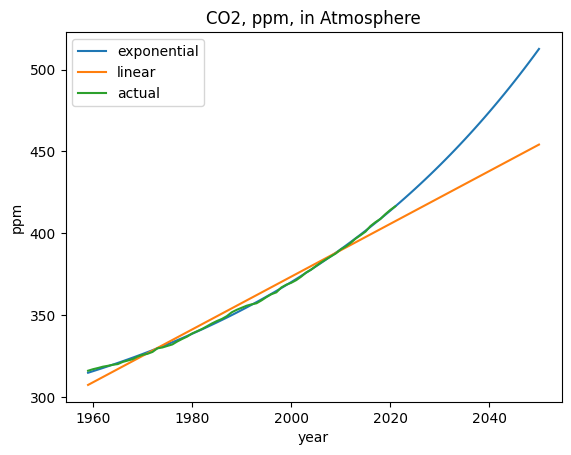
\includegraphics[width=\textwidth]{exponential}%
            \captionof{figure}{Graph of Exponential Regression}
            \label{fig:co2_exp}
        \end{minipage}%
        \begin{minipage}{0.3\linewidth}
            \centering
            \begin{tabular}{ll}
                \toprule
                Metric               & Value   \\
                \midrule
                MSE                  & 0.48061 \\
                RMSE                 & 0.69326 \\
                MAE                  & 0.56981 \\
                PCC                  & 0.99973 \\
                R\textsuperscript{2} & 0.99945 \\
                CVAR                 & 890.45  \\
                \bottomrule
            \end{tabular}
            \vspace{8pt}
            \caption{Error Metrics for Exponential Regression}
            \label{tab:co2_exp_err}
        \end{minipage}
    \end{table}

    Visually, the exponential function better aligns with the actual values; the predicted values also seem to fit with the general trend, and this is confirmed by extremely good error metrics, as show in Table~\ref{tab:co2_exp_err}.
    An advantage of exponential regression as a predictive model is that it provides high quality forecasts, which increase the accuracy of predicted values during interpolation.
    However, a key drawback is that a large data set is necessary to carry this method out, as a reasonable amount of continuity is needed to accurately predict future values, especially during extrapolation.

    \subsection{Sigmoid}
    The third predictive model selected shares similarities with the exponential model.
    While most sigmoid functions, when the domain is restricted, may behave very similar to an exponential function, the difference is that sigmoid functions also have an upper asymptote.
    The function has a S-shaped curve, comparable to two exponential functions, one with a negative exponent and one with a positive exponent, that are joined at the point of inflection.
    Sigmoid functions are commonly used to model growth variables with a natrual limit.
    The most common sigmoid function is the logistic function, which takes the general form of:
%
    \begin{equation}
        f(x) = \frac{L}{1 + e^{-k(x - x_0)}}
        \label{eq:logi}
    \end{equation}
%
    where
    $L$ is the curve\textquotesingle s maximum value,
    $k$ is the logistic growth rate, and
    $x_0$ is the x value of the sigmoid midpoint.

    The standard logistic function is, however, pretty limited; the minimum asymptote is fixed at zero and the shape of the curve is fixed other than the growth rate, which reflects the gradient at the midpoint.
    In order to fit to the CO\textsubscript{2} dataset, a more generalized and adjustable sigmoid function is used:
%
    \begin{equation}
        f(x) = \frac{x-x_{0}}{\left(s^{-z}+\frac{2\left|x-x_{0}\right|}{y_{max}-y_{min}}^{z}\right)^{\frac{1}{z}}}+\frac{y_{max}-y_{min}}{2}+y_{min}
    \end{equation}
%
    where
    $x_0$ is the x value of the sigmoid midpoint,
    $s$ is the growth rate or slope at the midpoint,
    $z$ governs the shape of the curve,
    $y_{max}$ is the maximum y value, and
    $y_{min}$ is the minimum y value.

    Removing parameters that allow linear transformations, the sigmoid function can be simplified to:
%
    \begin{equation}
        f(x) = \frac{x}{\left(s^{-z}+\frac{\left|x\right|}{L}^{z}\right)^{\frac{1}{z}}}
    \end{equation}
%
    and by removing the $z$ parameter, a basic algebraic sigmoid function remains:
%
    \begin{equation}
        f(x) = \frac{x}{s^{-1}+{\left|x\right|}/{L}}
    \end{equation}

    The function\textquotesingle s parameters were then manually adjusted to best suit the current data set, giving the following equation: ${y = 2523.6 / (1 + e^{(-0.017587 * (x - 2175.5))}) + 260.0180641636529}$. {y} was then set to 685 to find the year at which CO\textsubscript{2} emissions would reach 685ppm, it was found that it would reach this level at the year 2193. The equation was then graphed alongside with the regression lines of the two previous models to obtain the following graph:

    \begin{table}[h]
        \begin{minipage}{0.7\linewidth}
            \centering
            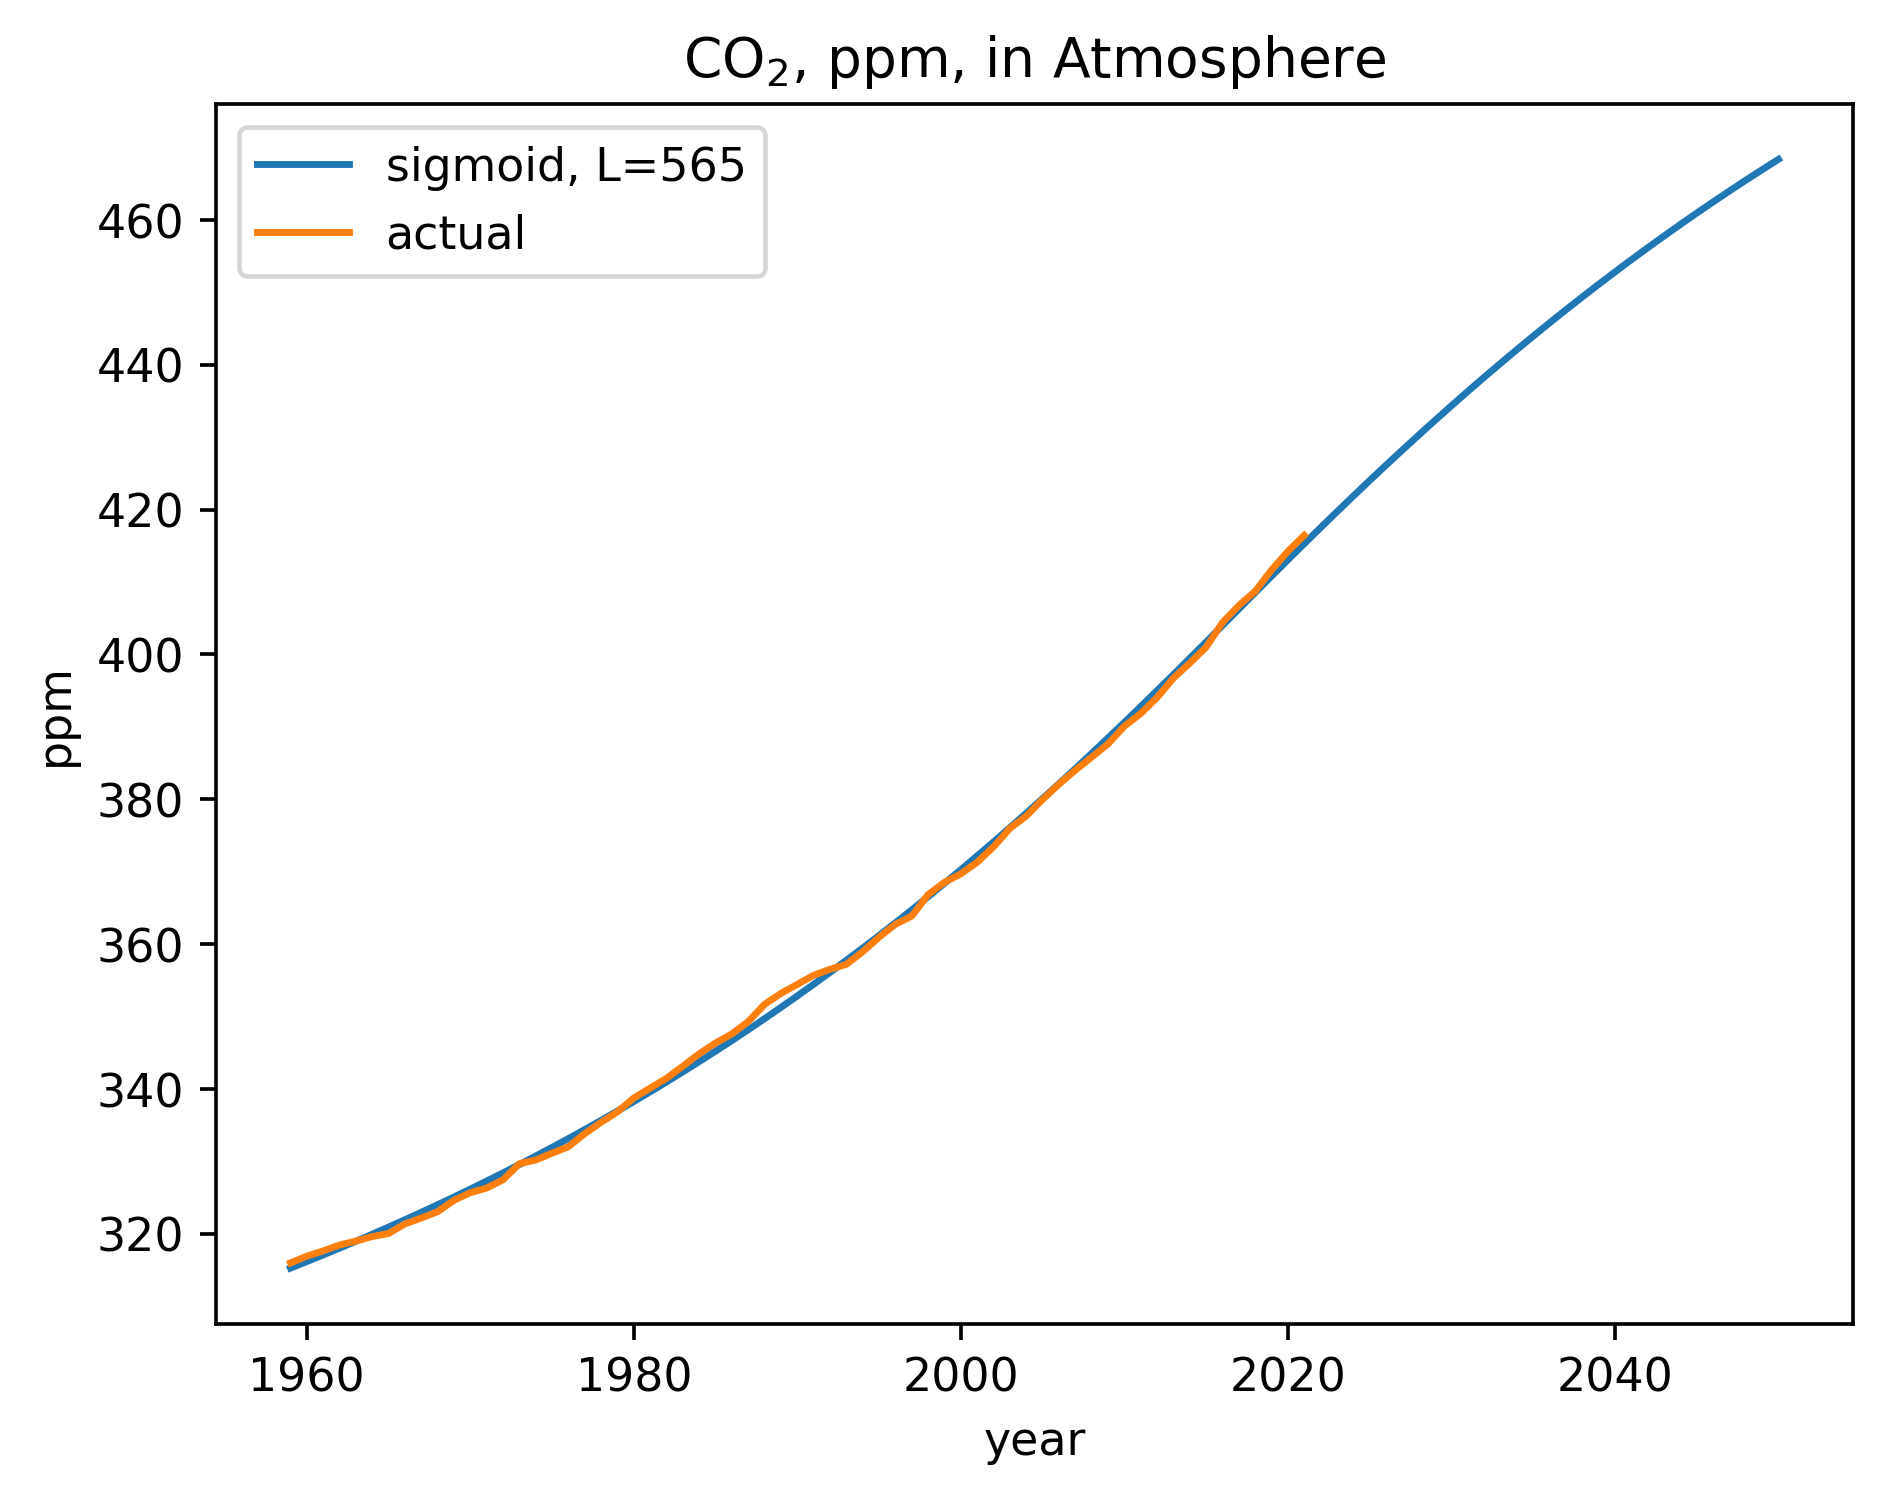
\includegraphics[width=\textwidth]{co2_sigm_565}%
            \captionof{figure}{Graph of Sigmoid Regression}
            \label{fig:co2_logi}
        \end{minipage}%
        \begin{minipage}{0.3\linewidth}
            \centering
            \begin{tabular}{ll}
                \toprule
                Metric               & Value   \\
                \midrule
                MSE                  & 0.61002 \\
                RMSE                 & 0.78104 \\
                MAE                  & 0.66351 \\
                PCC                  & 0.99965 \\
                R\textsuperscript{2} & 0.99930 \\
                CVAR                 & 889.87  \\
                \bottomrule
            \end{tabular}
            \vspace{8pt}
            \caption{Error Metrics for Sigmoid Regression}
            \label{tab:co2_logi_err}
        \end{minipage}
    \end{table}

    As can be seen, the logistic curve follows a very similar path to that of the exponential function. However, the 1959--2050 year range is too small to depict the sigmoid point, so the functions were graphed to reach the year 2400:

    \begin{center}
        \frame{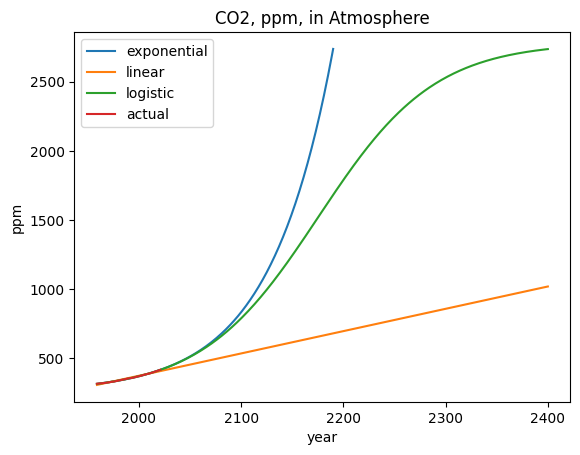
\includegraphics[scale=0.6]{logistic_2400}}
    \end{center}

    \subsection{Prophet}
    Prophet is a non-linear regression model released by Facebook, it is a procedure for forecasting time series data, working best with series that have strong seasonal effects of historical data. The graph for CO\textsubscript{2} levels over time can be plotted. The regression model is in the form:

    ${\displaystyle y_t = g_t + s_t + h_t +\epsilon_t}$

    Where:
    \begin{itemize}
        \item ${g_t}$ = Piecewise-linear trend
        \item ${s_t}$ = Seasonal patterns
        \item ${h_t}$ = Holiday effects
        \item ${\epsilon_t}$ = White noise error
    \end{itemize}

    \begin{center}
        \frame{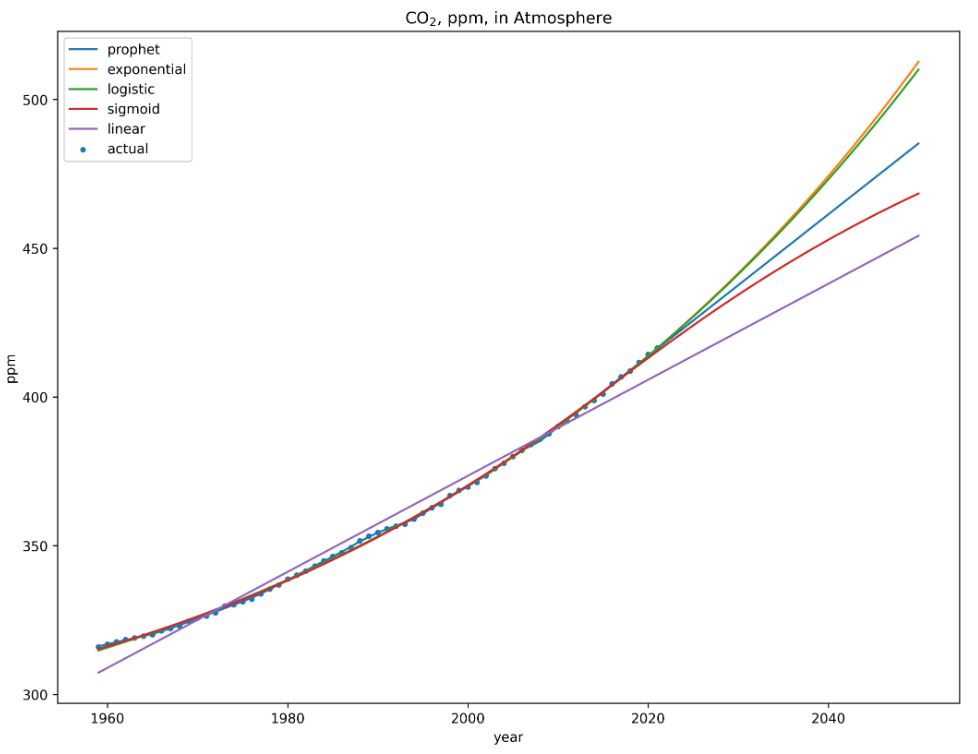
\includegraphics[scale=0.5]{prophet}}
    \end{center}

    Prophet is fast and generally maintains a high accuracy when predicting values. It can be used in a range of different contexts and it is robust to outliers, shifts in the overall trend and missing data. A key disadvantage is that a larger set of data is needed to accurately depict a trend-line.

    \subsection{ARIMA}
    An additional time-series prediction model that was investigated was ARIMA, which is based on ARMA (AutoRegressive Moving Average). These models are widely used in datasets that demonstrate non-stationarity, where the series\textquotesingle statistical properties such as mean, variance and autocorrelation change over time. ARIMA assumes the input data to be stationary, so any non-stationary data has to be made stationary through a reversible process. Usually, the transformation involves finding the general trend with methods such as regression and then using differencing to remove the trend from the dataset. With the trend eliminated, an ARIMA model can then be constructed and its optimal parameters found.

    Another appropriate model to use in regards to the data set is ARIMA. ARIMA models are generally denoted as ARIMA (p, d, q) where:
    \begin{itemize}
        \item p = Number of Auto-Regressive (AR) terms
        \item d = Number of differencing
        \item q = Number of Moving Average (MA) terms
    \end{itemize}

    The functions AR(p) and MA(q) are defined below as:

    -----------THERES SUPPOSED TO BE A TABLE HERE----------

    Before tuning the parameters p and q, the number of differencing required to make the data stationary must be found out. To evaluate whether the current dataset is stationary, an Augmented Dickey-Fuller (ADF) test was performed.

    ADF tests expand on the original Dickey-Fuller test by including higher-order autoregressive processes to form the equation given below:

    ${\Delta y_{t}=\alpha +\beta t+\gamma y_{t-1}+\delta _{1}\Delta y_{t-1}+\cdots +\delta _{p-1}\Delta y_{t-p+1}+\varepsilon _{t}}$

    Where:
    \begin{itemize}
        \item ${y_{t}}$ = Value of the time series at time t
        \item ${\alpha}$ = constant
        \item ${\beta}$ = Coefficient on a time trend
        \item {p} = Lag order of autoregressive process
    \end{itemize}

    The results of the ADF test applied on the given dataset is presented below:

    -------THERES SUPPOSED TO BE ANOTHER TABLE HERE---------

    The p-value obtained is greater than the significance level 0.05 and the ADF statistic is higher than any of the critical values, hence it can be concluded that the time series has a unit root and is non-stationary. The high p-value signifies that a high order of differencing will need to be used.

    To further confirm the data\textquotesingle s stationarity, autocorrelation and partial autocorrelation graphs were also used. AFC and PAFC functions are measures of correlation between past and present data, and indicate which past data values are most useful in predicting future ones. The results of these functions are then used to select the most optimal parameters for p and q. Both functions were applied on the given dataset and the graphed results displayed below:

    \begin{center}
        \frame{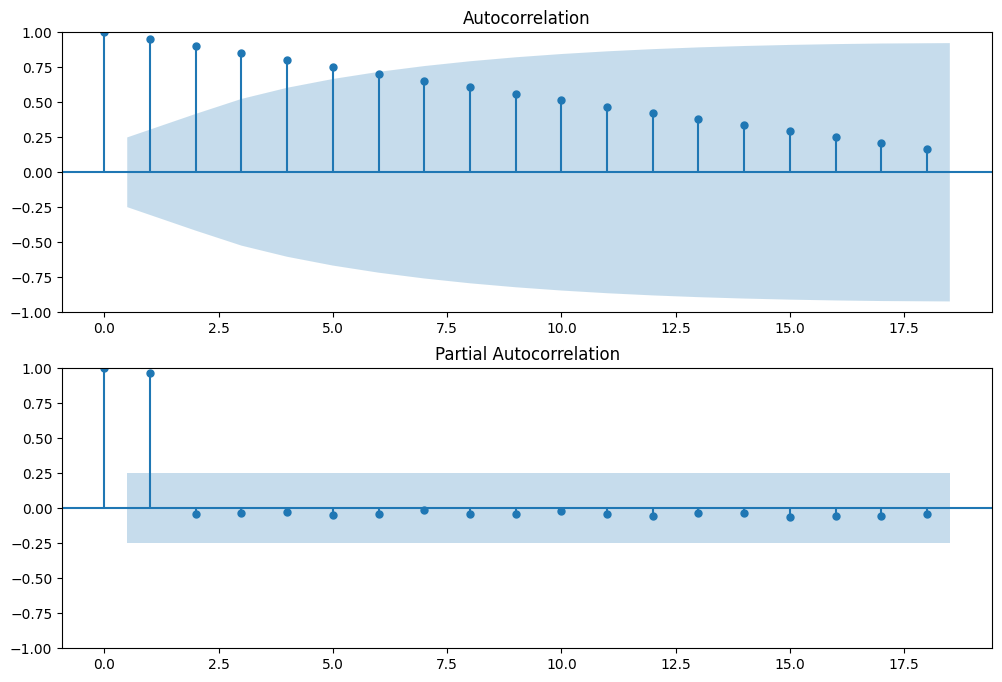
\includegraphics[scale=0.5]{pacf_acf}}
    \end{center}

    For both graphs the x-axis represents lag, whereas the y-axis indicates the correlation strength. ACF graphs represent the correlation between data values that are n intervals apart. PACF graphs are similar in that they represent the same information, however they also account for the values of the intervals in between.

    The correlation that can be seen in the AFC graph is negative, indicating that large current values correspond with small values at the specified lag. The absolute correlation values represent the strength of the relationship; to construct an ARIMA model, the expected trend of these values should be random. In this case, the initial relationship between past and present values is strong, but gradually decreases over lags, indicating a clear trend of decreasing correlation strength.

    If the autocorrelation follows a random non-linear trend, then AR(p) and MA(q) can be applied to the graphed functions to obtain the optimal parameter values for p and q.
    However, this is only assuming the data does not have a trend or seasonality component, which does not apply to the given dataset.

    The autocorrelation trend as well as the high order of differencing required to transform the data to stationary (as seen in the ADF test) both demonstrate that the given dataset is unsuitable for constructing an ARIMA model, and therefore this prediction model has been rejected and will not be used as part of the predicted CO\textsubscript{2} and temperature values.


    \section{CO\textsubscript{2} - Model Evaluation}
    To rank the 4 accepted predictive models on their mathematical accuracy, the following error metrics are to be calculated for each model and then compared with each other:

    --------------ANOTHER TABLE---------------------------

    \subsection{Procedure}
    \noindent \textbf{Separation of Known Values into Testing and Training data}

    75\% of known data values are allocated to the testing data group, remaining 25\% are allocated to the training group. The predictive model will take in the training group data values as its sole input, and will predict the remaining 25\%. The model\textquotesingle s predicted values are then to be compared with the training group\textquotesingle s values and the forecast errors obtained.
    A forecast error is defined as the difference between an observed and its forecasted value; the formula for a single forecast error can be modified to suit multiple data values, and it is denoted by the following equation:
    q1
    ${e_{T+h} = y_{T+h} - \hat{y}_{T+h|T}}$

    Where:
    \begin{itemize}
        \item ${e_{T+h}}$ = Forecast error
        \item ${y_{T+h}}$ = Actual value of the h-step observation
        \item ${\hat{y}_{T+h|T}}$ = Actual value of the h-step forecast
    \end{itemize}


    [ADD GRAPHED RESULTS HERE + CALCULATED FORECAST ERRORS]

    It is important to note that although a model may fit the training data well, it does not necessarily mean the model will forecast well, therefore it is important to take the other error metrics into consideration.

    \subsection{Accuracy Analysis}

    \subsubsection*{MSE}
    Mean Squared Error (MSE) is a measure of the quality of a predictor or of an assessor, its definition differing accordingly. It is the average squared distance between the actual and predicted values, measuring the variance of the residuals. In this case, only the quality of the predictor is to be assessed. It involves taking the average squared distance between the actual and predicted values, measuring the variance of the residuals. The within-sample MSE of a predictor can then be denoted as:

    ${\operatorname {MSE} ={\frac {1}{n}}\sum _{i=1}^{n}\left(Y_{i}-{\hat {Y_{i}}}\right)^{2}}$

    Where:
    \begin{itemize}
        \item ${\frac {1}{n}\sum _{i=1}^{n}}$ = Mean
        \item ${\left(Y_{i}-{\hat {Y_{i}}}\right)^{2}}$ = Squares of the errors
    \end{itemize}

    MSE also has a differentiable graph so it makes it easier to perform mathematical operations in comparison to MAE. MSE is more sensitive to outliers compared to MAE\@.

    \subsubsection*{RMSE}
    Root Mean Squared Error (RMSE) is the square root of the MSE, measuring the standard deviation of the residuals. The higher the RMSE value, the larger the deviation between actual and predicted values. By proxy, the lower the RMSE value, the lower the deviation, hence the model is more accurate. Building on the last error metric formula, RMSE can be denoted as:

    ${\operatorname {RMSE} = \sqrt{MSE}}$

    When outliers are exponentially rare, such as this situation, RMSE is generally preferred over MSE as it provides a better evaluation of model performance, as it uses the same units as the Y axis (CO\textsubscript{2} emissions).

    \subsubsection*{MAE}
    Mean Absolute Error (MAE) is the sum of the absolute difference between the actual and predicted values. A perfect prediction model would yield a 0 as its MAE value. The further away from 0 the MAE value is, the more errors the model makes and hence the less accurate the model is. The formula to calculate MAE is denoted as:

    ${\displaystyle {MAE} ={\frac {\sum _{i=1}^{n}\left|y_{i}-x_{i}\right|}{n}}}$

    Where:
    \begin{itemize}
        \item ${\sum _{i=1}^{n}\left|y_{i}-x_{i}\right|}$ = Sum of absolute error
        \item {n} = Number of errors
    \end{itemize}

    \subsubsection*{PMCC, ${R^2}$ AND COVARIANCE}
    The last 3 error metrics are explained in further detail when exploring the relationship between temperature and CO\textsubscript{2} emissions

    \subsubsection*{Results}
    The MSE, RMSE, MAE, PMCC, R\textsuperscript{2} and covariance were calculated for each accepted model, rounded to 5 s.f, and compiled into a results table below. For each error metric, the model with the value closest to and furthest from a perfect value were highlighted:

    ---------------A TABLE, AGAIN.-------------------
    --------------LO AND BEHOLD, ANOTHER TABLE--------------

    \subsection{Overall Evaluation}

    \noindent\textbf{Strength 1}: asdf

    \noindent\textbf{Strength 2}: asdf

    \noindent\textbf{Weakness 1}: asdf

    \subsection{Possible Improvements}
    blah blah

    \newpage


    \section{CO\textsubscript{2} - Results \& Conclusions}

    \subsection{Forecast Results}
    we\textquotesingle re doomed

    \subsection{Comparison with External Claims}
    they\textquotesingle re all wrong


    \section{Temperature - Modelling}

    \subsection{Time Series}
    Temperature over time.

    \subsection{Relationship with CO\textsubscript{2}}
    100\% causation


    \section{Temperature - Model Evaluation}

    \subsection{Predictive Ability}
    our model definitely retains its accuracy 1000 years into the future.


    \section{Temperature - Results \& Conclusions}

    \subsection{Forecast Results}
    time to get baked.


    \section{References}

    \subsection{Program Code}
    \noindent Result data generated:
    \begin{verbatim}
    text data stuff

    \end{verbatim}

    \noindent Python program code:
    \begin{lstlisting}[language=Python]
        # pass

    \end{lstlisting}

    \subsection{Bibliography}
%    \printbibliography

\end{document}
